\begin{frame}
\frametitle{Depth Testing: Demo}

\begin{columns}

\column{.5\textwidth}

\begin{figure}[ht]
    \centering
    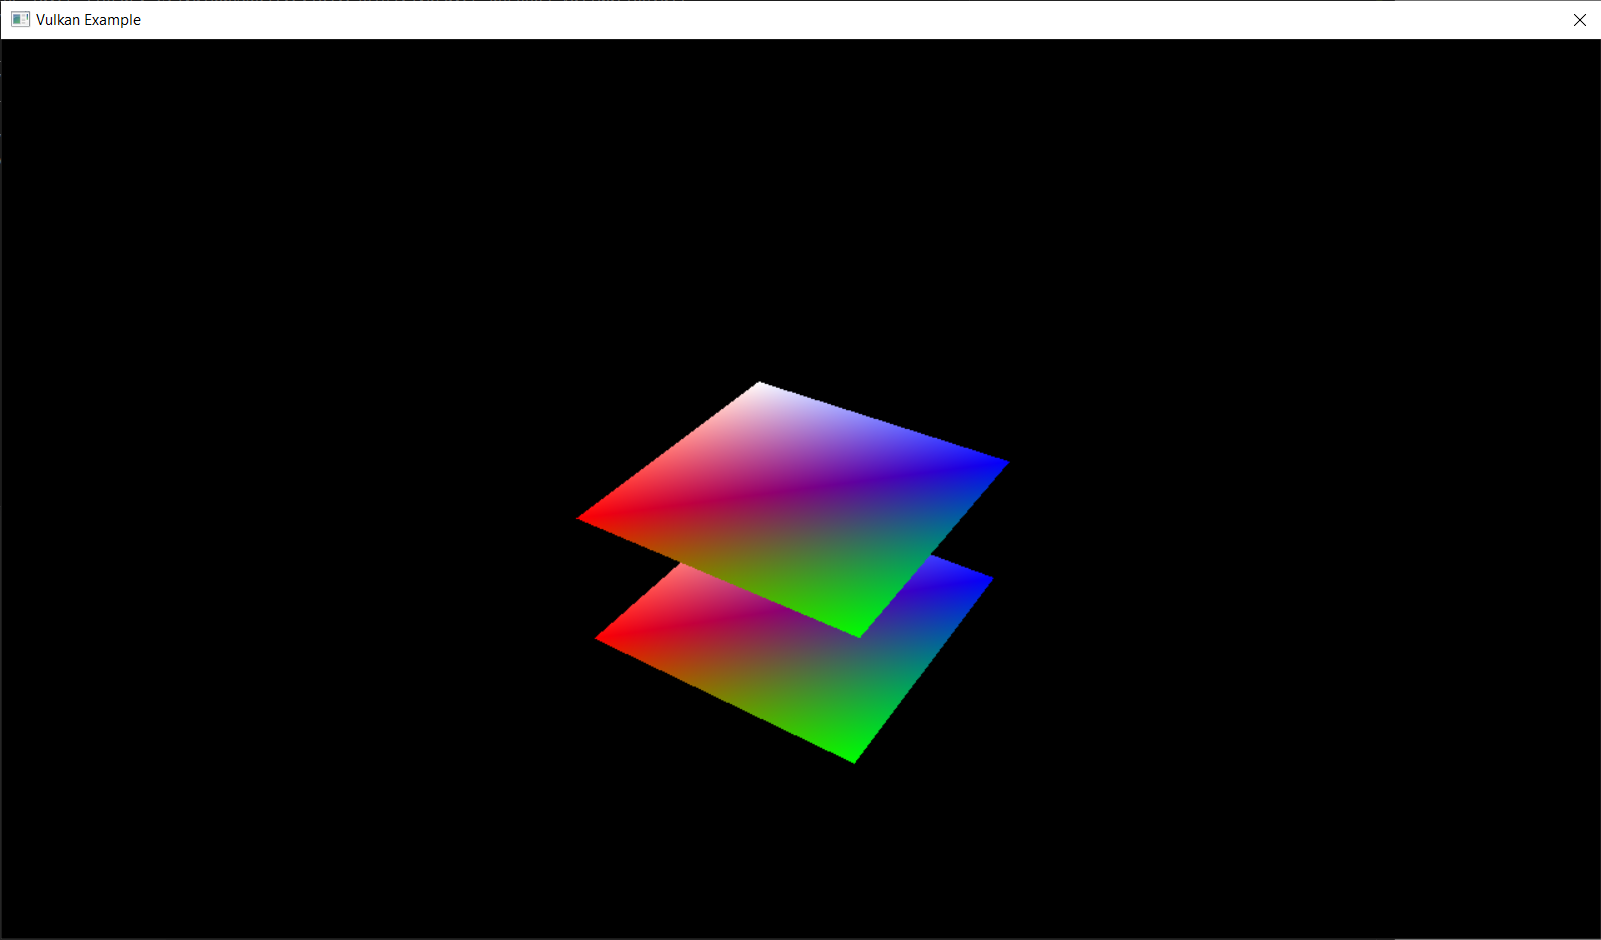
\includegraphics[scale=0.14]{images/SlidesDepthTesting/DepthTesting.png}
\end{figure}

\column{.5\textwidth}

\begin{figure}[ht]
    \centering
    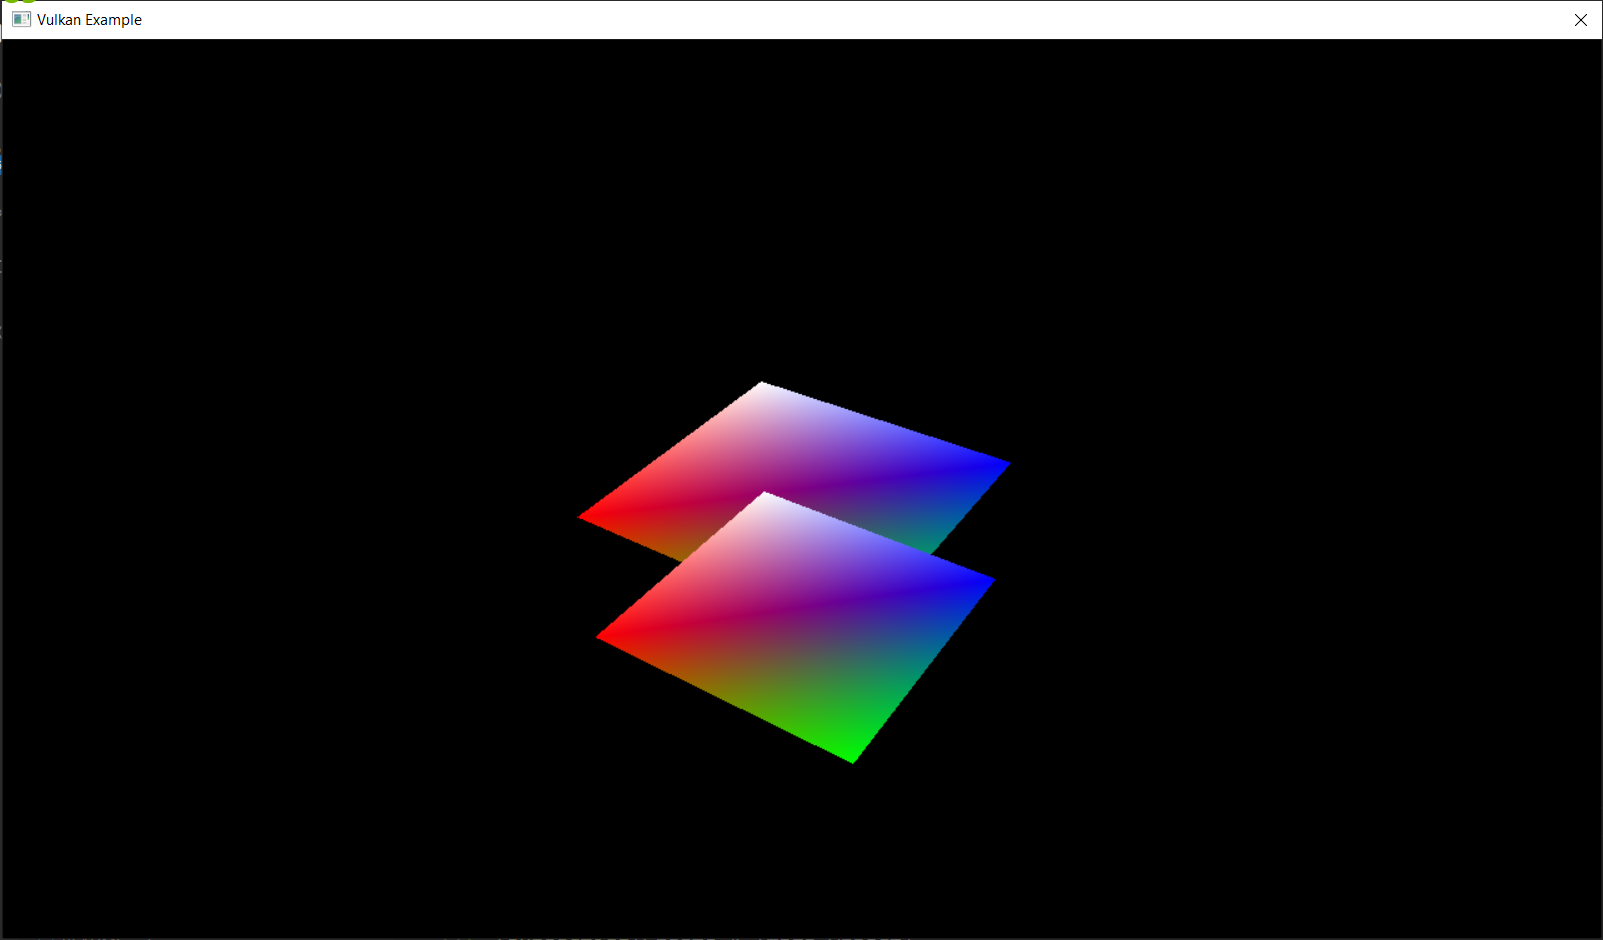
\includegraphics[scale=0.14]{images/SlidesDepthTesting/NoDepthTesting.png}
\end{figure}

\end{columns}

\end{frame}

\begin{frame}
\frametitle{Depth Buffer: Idea}
\begin{itemize}
\item Come renderizzare oggetti in modo tale che quelli più vicini possano nascondere quelli più lontani?
\item Possiamo ordinare gli oggetti in base alla loro lontananza dal punto di vista
\item Questa soluzione non funziona bene se due o più oggetti si sovrappongono in tutto o in parte
\item Se gli oggetti da renderizzare sono opachi, allora possiamo usare un depth buffer
\item Un depth buffer è un'immagine che codifica informazioni riguardanti la distanza dei frammenti dal punto di vista
\item Quando un frammento viene generato, compariamo la profondità del frammento con quella salvata nel corrispettivo texel del depth buffer
\item Se è più grande, il frammento non viene utilizzato
\item Se è più piccola, il frammento viene utilizzato e la sua profondità viene salvata nel depth buffer
\end{itemize}
\end{frame}

\begin{frame}
\frametitle{Depth Buffer: Implementazione}
\begin{itemize}
\item Allochiamo un'immagine, sulla memoria della GPU, che possa essere usata come depth buffer
\item Nel nostro render pass, aggiungiamo un nuovo attachment
\item Questo attachment viene usato come depth stencil attachment durante il nostro subpass
\item Quando creiamo un framebuffer, dobbiamo ricordarci di aggiungere l'immagine che funge da depth buffer
\item Durante la creazione del pipeline state object dobbiamo abilitare il depth testing
\item Quando iniziamo un'istanza del render pass, specifichiamo un clear value di $1.0$ per il depth buffer
\end{itemize}
\end{frame}
